\section{Java-Web-Anwendungen} \label{sec:tech-WebAnwendungen}
		\subsection{Java Server Faces - JSF}
		
Nach \citep{Bill2004} ist JavaServer Faces (JSF) ein komponenten-abh�ngiges Web-Framework, mit dessen Hilfe sich Benutzerschnittstellen mit einer Reihe von wiederverwendbaren GUI-Komponenten, z.B. Labels, Buttons, Eingabefelder usw.,einfach erstellen lassen. JSF ist ein erster offizieller Standard von Sun hinsichtlich der Erstellung von UIs\footnote{User Interface (engl. Benutzerschnittstelle)} von Webanwendungen und wurde im Rahmen des Java Community Process (JCP) unter dem JSR 127\footnote{\url{http://www.jcp.org/en/jsr/detail?id=127}} im September 2002 ver�ffentlicht. Im Experten-Gremium sind viele namhafte Firmen wie IBM, BEA, IONA, Novell, Borland, HP, Oracle oder Siemens, was eine gro�e Unterst�tzung seitens der Industrie erwartet.

\begin{figure}[h]
	\centering
	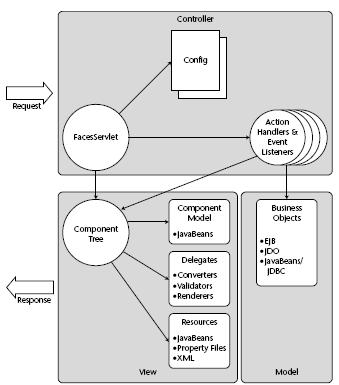
\includegraphics[scale=1]{images/Architektur-JSF.jpg}
	\caption{Architektur von JSF \citep[Bild 1.6]{Bill2004}}
	\label{fig:architecture_jsf}
\end{figure}

Die auf dem bekannten Model View Controller 2(MVC2)-Modell basierende JSF-Technologie besteht aus den folgenden zwei Hauptkomponenten:

\begin{itemize}
	\item JSF API
	\item JSF Tag Libraries
\end{itemize}

Das Pr�sentations-Framework JSF muss die von MVC definierten Komponenten abbilden. Wie in \vref{fig:architecture_jsf} zu sehen ist, wird das Modell durch einfache JavaBeans, aber auch durch EJBs\footnote{Enterprise Java Beans} oder JDOs\footnote{Java Data Objects} abgebildet. Der Controller wird durch Action Handler bzw. Event Listener der jeweiligen UI-Komponenten dargestellt. Im Zentrum des Controllers steht das FacesServlet, welches mit Hilfe der Konfiguration reagieren, agieren und navigieren kann. JSPs und Komponenten sowie deren Renderer, Converter und Validatoren bilden die Views ab. In jeder View, welche meistens durch eine JavaServer Page (JSP) aufgebaut ist, existiert ein entsprechender Component Tree. Dieser beinhaltet alle Komponenten, die in der JSP durch definierte Tags dargestellt werden. Somit hat der Entwickler Zugriff auf alle Komponenten im Laufe des Lebenszyklus der Request-Bearbeitung.\\

Dieser Lebenszyklus wird zu jeder Anfrage an die JSF-Applikation durchlaufen und enth�lt folgende Phasen:
 
\begin{enumerate}
	\item Restore View: Aufbau des Component Tree
	\item Apply Request Values: Die Daten aus dem Request werden den Komponenten zugeordnet
	\item Process Validations: Die Variablen der Komponenten werden validiert
	\item Update Model Values: Die Variablen der Komponenten werden in deren Datenmodellen gespeichert
	\item Invoke Application: Ausf�hrung der Business-Logik
	\item Render Response: Der Component Tree wird aktualisiert und ein Response generiert
\end{enumerate}		

Die Navigation in einer JSF-Applikation wird in einer Konfigurationsdatei definiert. Darin ist f�r jede JSP jeweils eine Navigationsregel festgelegt. Diese Regeln bestehen aus der Aufrufenden Seite sowie verschiedenen Navigationsf�llen. Solche Fallunterscheidungen machen die Navigation abh�ngig von den Ergebnissen der Businesslogik und sorgen f�r die Dynamik der Anwendung.\\

\textbf{Fazit:} Da in der Projektplanungsphase die derzeitige JSF-Spezifikation zwar relativ ausgereift war, aber noch nicht in einer Finalversion vorlag, wurde in der Phase der Implementierung auf dessen Verwendung verzichtet und stattdessen auf Apache Struts zur�ckgegriffen.

\newpage

\subsection{Apache Struts}



























%Hier danach nicht mehr schreiben
\label{sec:tech-WebAnwendungen-ende}